\documentclass{article}
\usepackage[utf8]{inputenc}
\usepackage{graphicx}
\usepackage{hyperref}
\setlength{\parindent}{0pt}
\setlength{\parskip}{1em}

\begin{document}

\section{User Acceptance Testing}

\textbf{8/11/19 - 10:50am}

For this User Acceptance Test (UAT) to pass it will need to:
\begin{enumerate}
    \item Extract body text from a .txt file and create a new .txt file with that text.
    \item Extract title text from a .txt file and create a new .txt file with that text.
    \item Extract title and subtitle text together from a .txt file and create a new .txt file with that text.
    \item Analyse the body text for word frequency and create a .csv file that has that information.
    \item Analyse the title text for word frequency and create a .csv file that has that information.
    \item Analyse the title and subtitle text for word frequency and create a .csv file that has that information.
\end{enumerate}

I have created a new .txt file for this UAT.

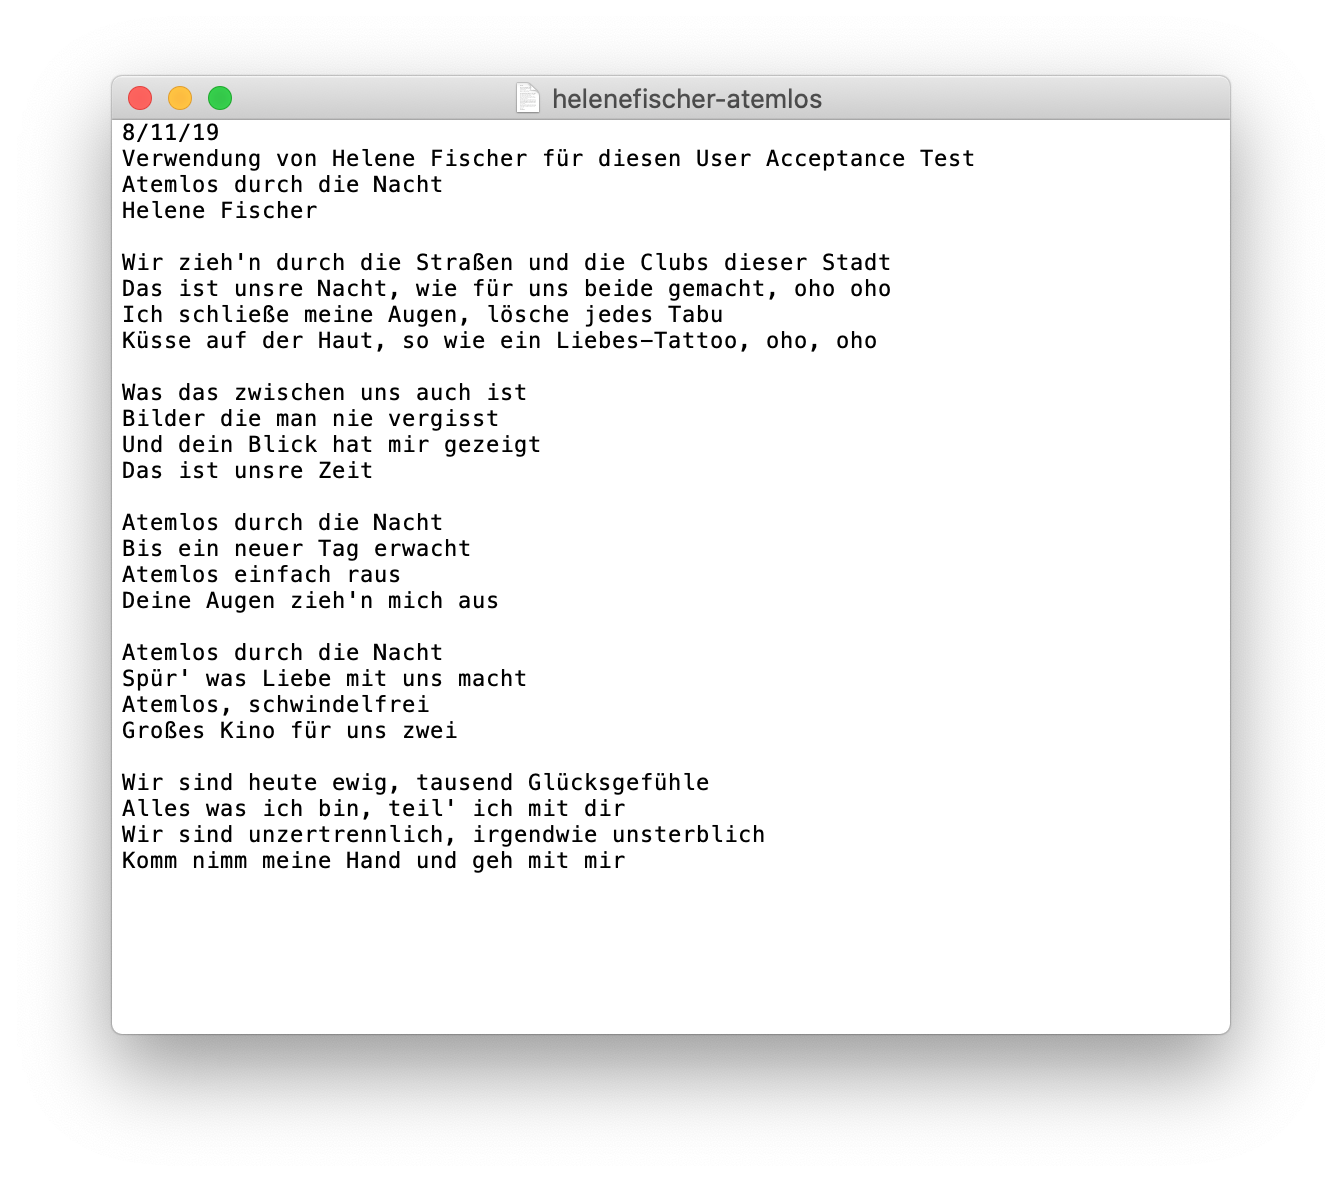
\includegraphics[width=\textwidth]{uat01.png}

I have also duplicated it 4 times so there are 5 copies of the same .txt file. This is to test if the Proof of Concept can accept multiple .txt files as a corpus.

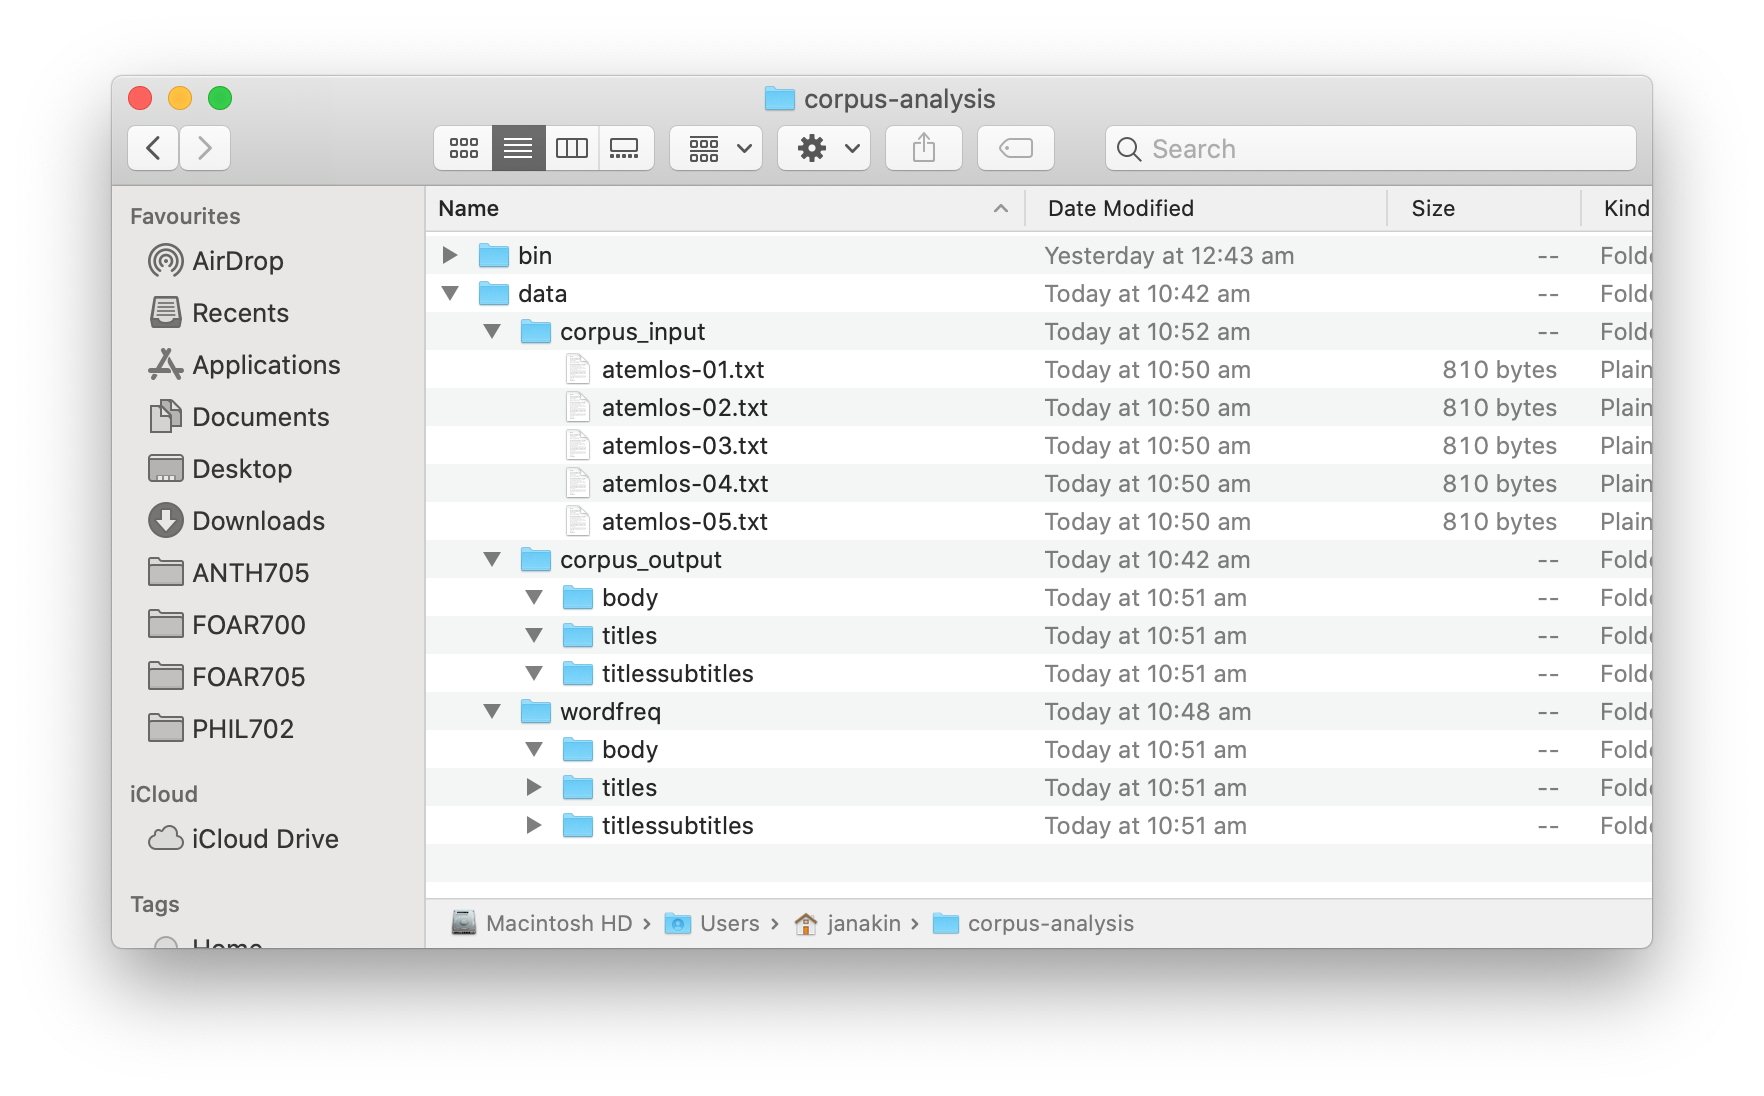
\includegraphics[width=\textwidth]{uat02.png}

Having counted the frequency of words in the body text lyrics I will use, I expect that it would yield the same results multiplied by 5.

\begin{itemize}
    \item atemlos - 20
    \item oho - 20
    \item nacht - 15
    \item ziehn - 10
    \item unsre - 10
    \item augen - 10
\end{itemize}

For the titles and titles and subtitles result I should expect no word over 5 as they only occur once.

Titles
\begin{itemize}
    \item verwendung - 5
    \item helene - 5
    \item fischer - 5
    \item user - 5
    \item acceptance - 5
    \item test - 5
\end{itemize}

Titles and Subtitles
\begin{itemize}
    \item verwendung - 5
    \item helene - 5
    \item fischer - 5
    \item user - 5
    \item acceptance - 5
    \item test - 5
    \item atemlos - 5
    \item nacht - 5
\end{itemize}

Now for the test.

\textbf{Objective:} Run UAT to see if Proof of Concept meets the Objective Criteria.

\textbf{Action:} Opened Terminal, navigated to the bin directory and called: \begin{verbatim}
    bash go.sh
\end{verbatim}

\textbf{Error:} None as such, but some warnings.

\textbf{Result:} This is what Terminal returned

\begin{verbatim}
Janakins-MBP:~ janakin$ cd corpus-analysis/bin
Janakins-MBP:bin janakin$ ls
delete.sh			go.sh
extractbody.sh			wordfreq_body.R
extracttitles.sh		wordfreq_titles.R
extracttitlessubtitles.sh	wordfreq_titlessubtitles.R
Janakins-MBP:bin janakin$ bash go.sh 
Loading required package: tm
Loading required package: NLP
Warning message:
In tm_map.SimpleCorpus(VCorpus, stripWhitespace) :
  transformation drops documents
Warning message:
In tm_map.SimpleCorpus(VCorpus_clean, content_transformer(tolower)) :
  transformation drops documents
Warning message:
In tm_map.SimpleCorpus(VCorpus_clean, removeWords, stopwords("german")) :
  transformation drops documents
Warning message:
In tm_map.SimpleCorpus(VCorpus_clean, removePunctuation) :
  transformation drops documents
Warning message:
In tm_map.SimpleCorpus(VCorpus_clean, removeNumbers) :
  transformation drops documents
Warning message:
In tm_map.SimpleCorpus(VCorpus_clean, removeWords, c("„", "—")) :
  transformation drops documents
Loading required package: tm
Loading required package: NLP
Warning message:
In tm_map.SimpleCorpus(VCorpus, stripWhitespace) :
  transformation drops documents
Warning message:
In tm_map.SimpleCorpus(VCorpus_clean, content_transformer(tolower)) :
  transformation drops documents
Warning message:
In tm_map.SimpleCorpus(VCorpus_clean, removeWords, stopwords("german")) :
  transformation drops documents
Warning message:
In tm_map.SimpleCorpus(VCorpus_clean, removePunctuation) :
  transformation drops documents
Warning message:
In tm_map.SimpleCorpus(VCorpus_clean, removeNumbers) :
  transformation drops documents
Warning message:
In tm_map.SimpleCorpus(VCorpus_clean, removeWords, c("„", "—")) :
  transformation drops documents
Loading required package: tm
Loading required package: NLP
Warning message:
In tm_map.SimpleCorpus(VCorpus, stripWhitespace) :
  transformation drops documents
Warning message:
In tm_map.SimpleCorpus(VCorpus_clean, content_transformer(tolower)) :
  transformation drops documents
Warning message:
In tm_map.SimpleCorpus(VCorpus_clean, removeWords, stopwords("german")) :
  transformation drops documents
Warning message:
In tm_map.SimpleCorpus(VCorpus_clean, removePunctuation) :
  transformation drops documents
Warning message:
In tm_map.SimpleCorpus(VCorpus_clean, removeNumbers) :
  transformation drops documents
Warning message:
In tm_map.SimpleCorpus(VCorpus_clean, removeWords, c("„", "—")) :
  transformation drops documents
Janakins-MBP:bin janakin$ 
\end{verbatim}

The files were created in the right areas.

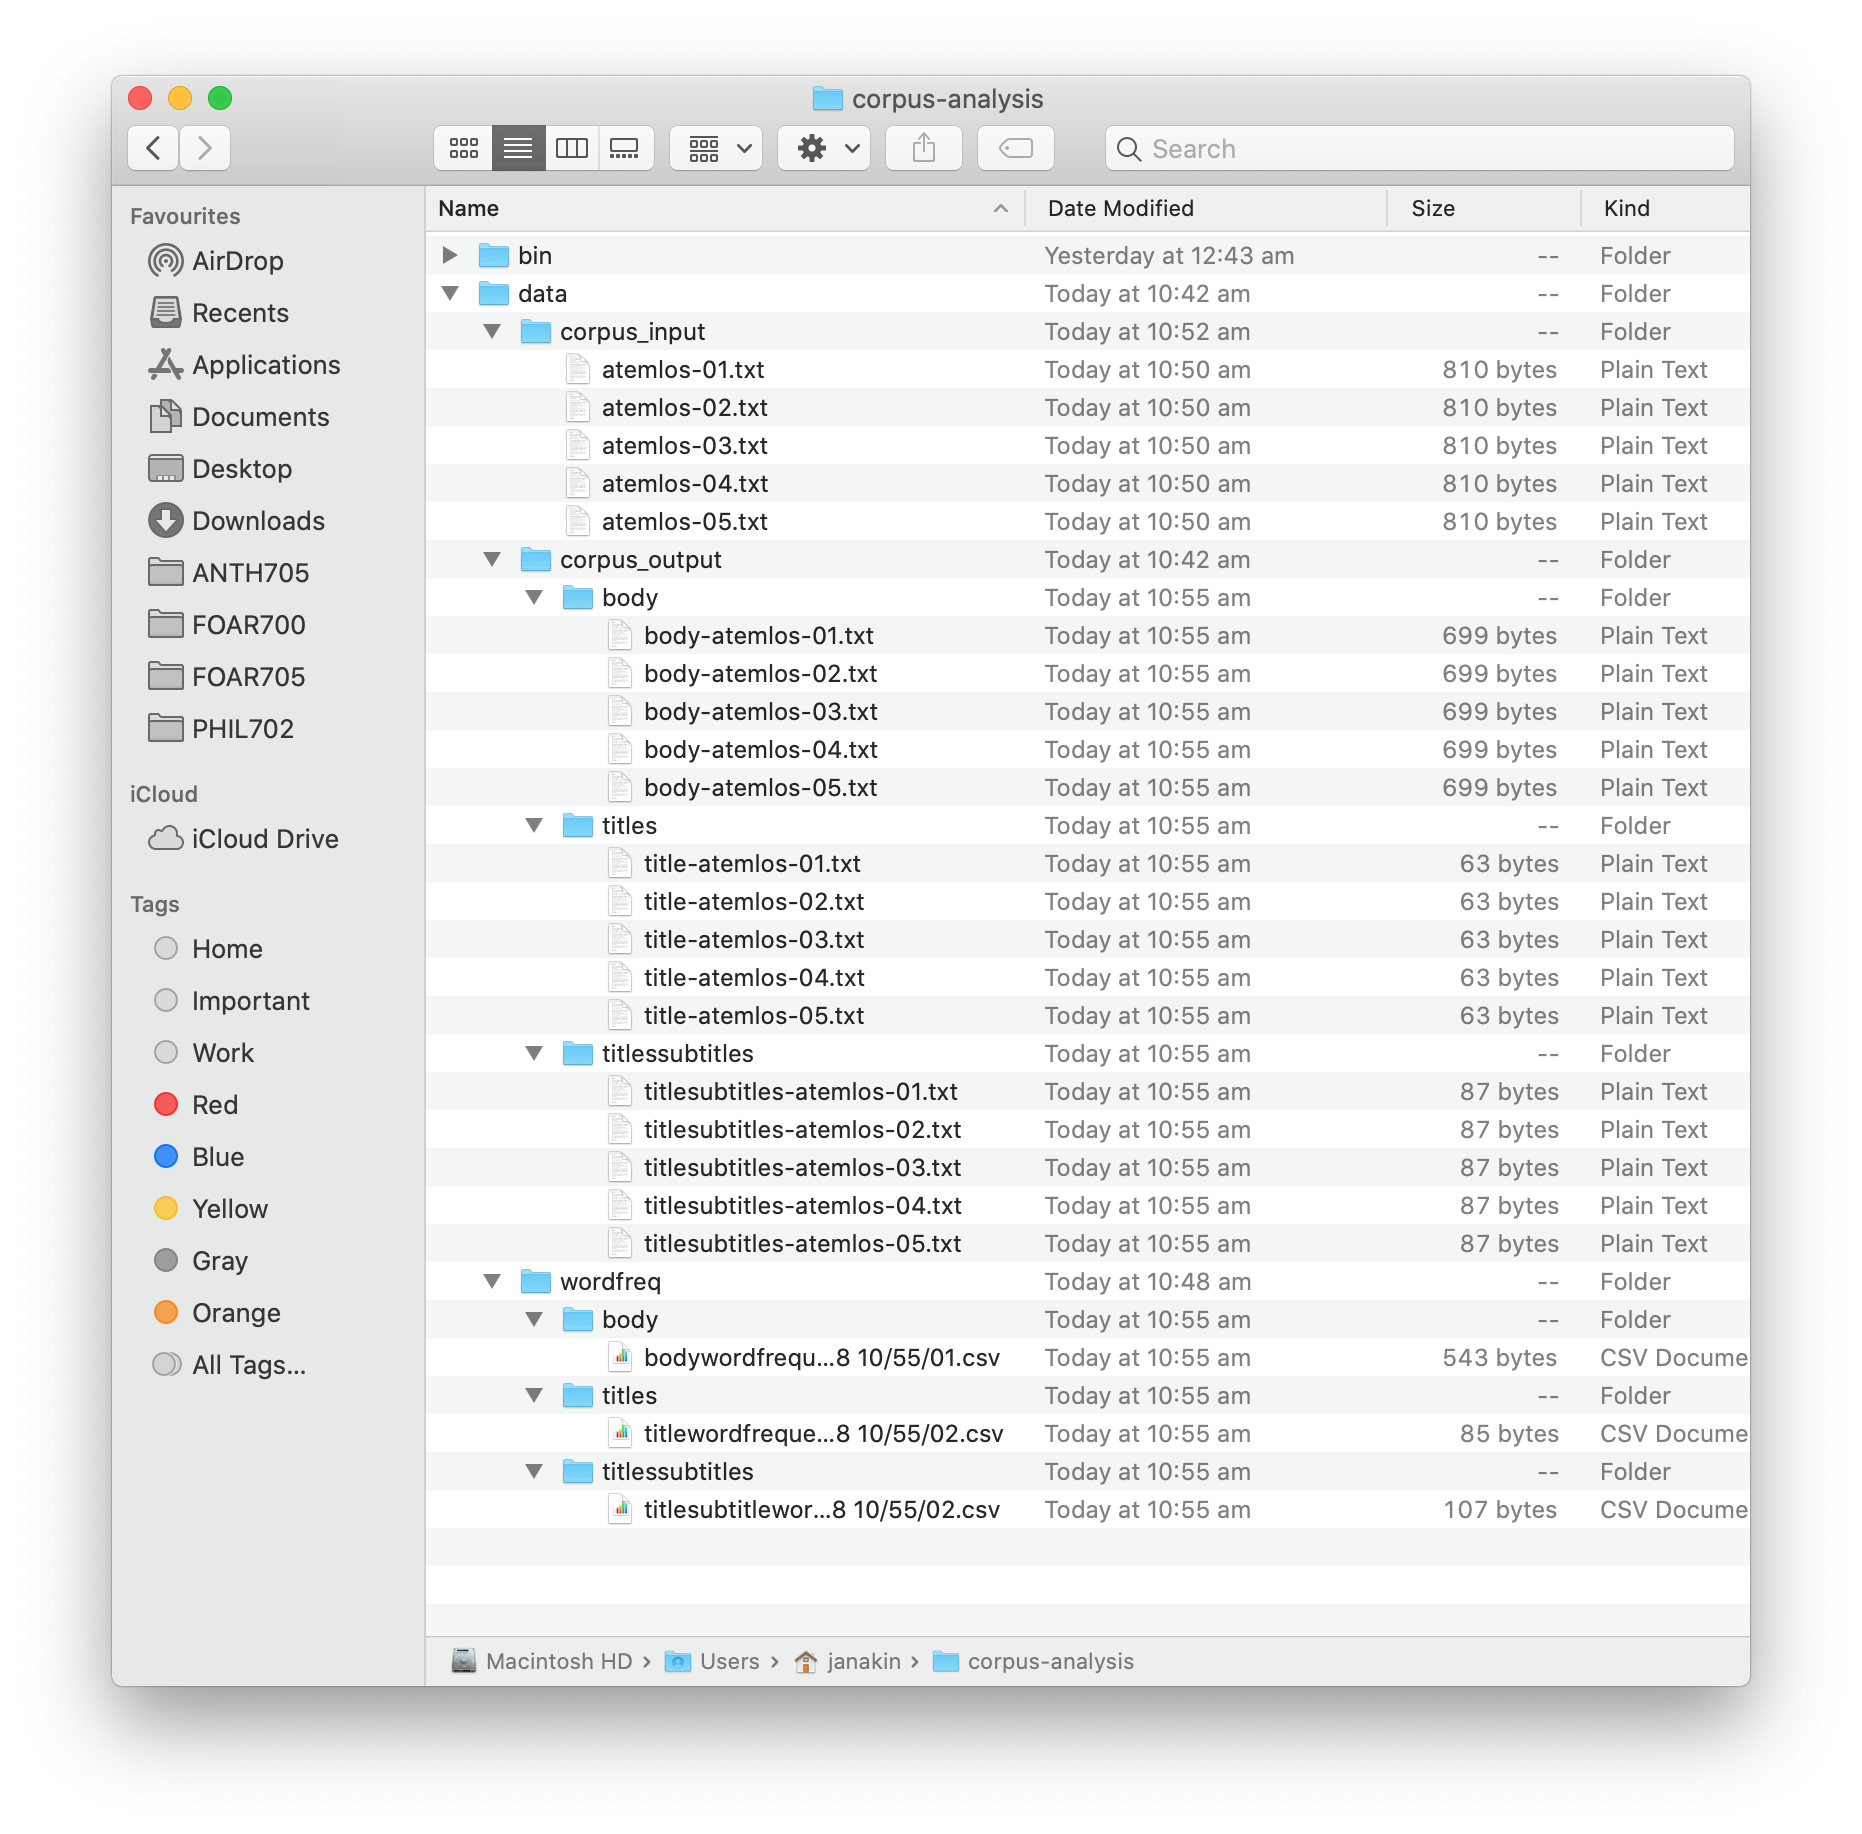
\includegraphics[width=\textwidth]{uat03.png}

The body text was extracted correctly.

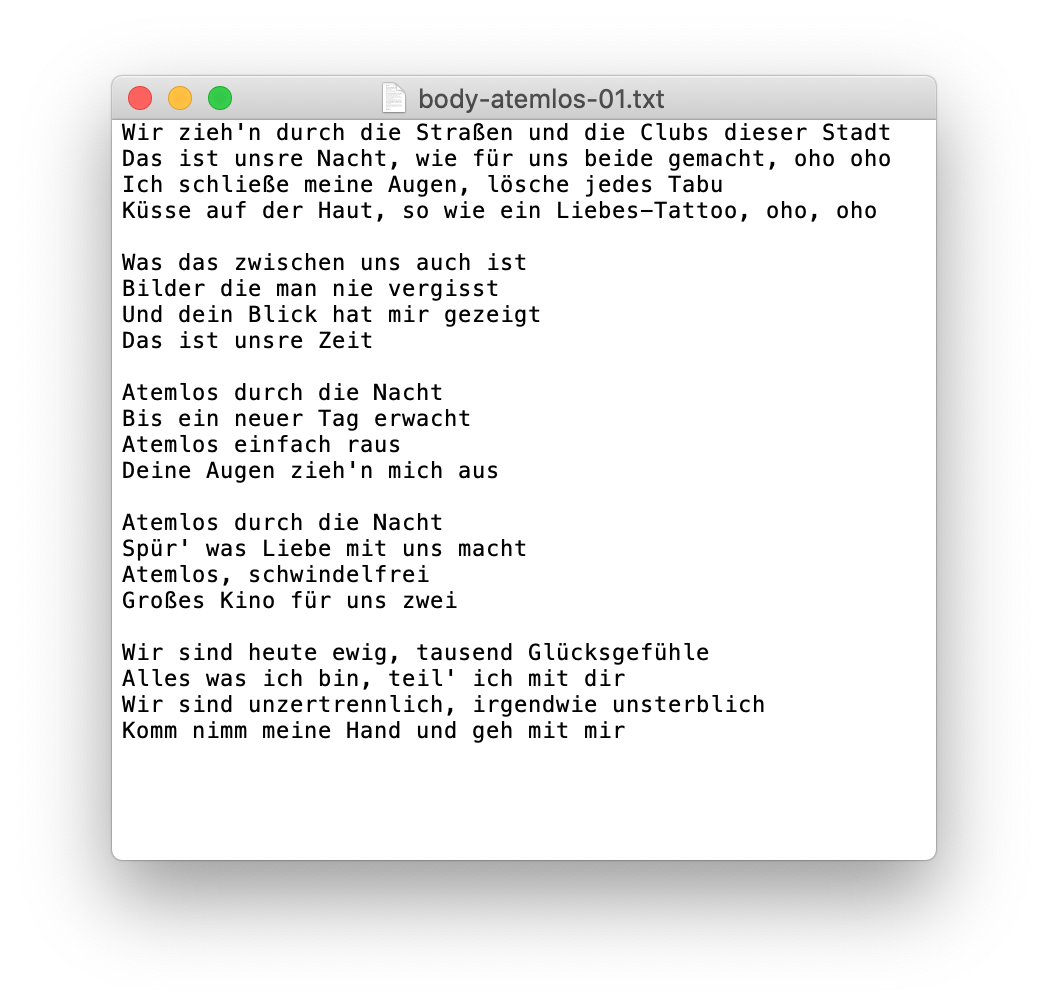
\includegraphics[width=\textwidth]{uat04.png}

The title text was extracted correctly.

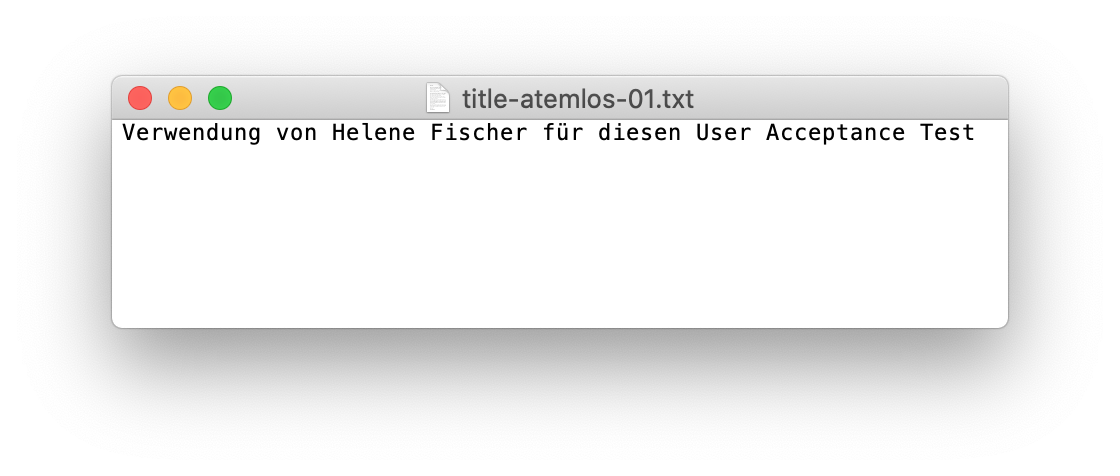
\includegraphics[width=\textwidth]{uat05.png}

The title and subtitle text was extracted correctly.

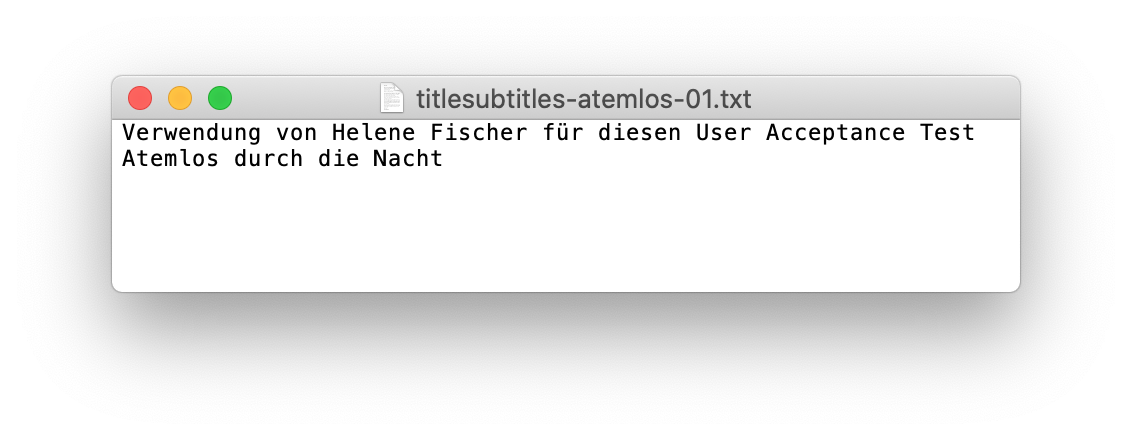
\includegraphics[width=\textwidth]{uat06.png}

Results from the body text frequency analysis are below.

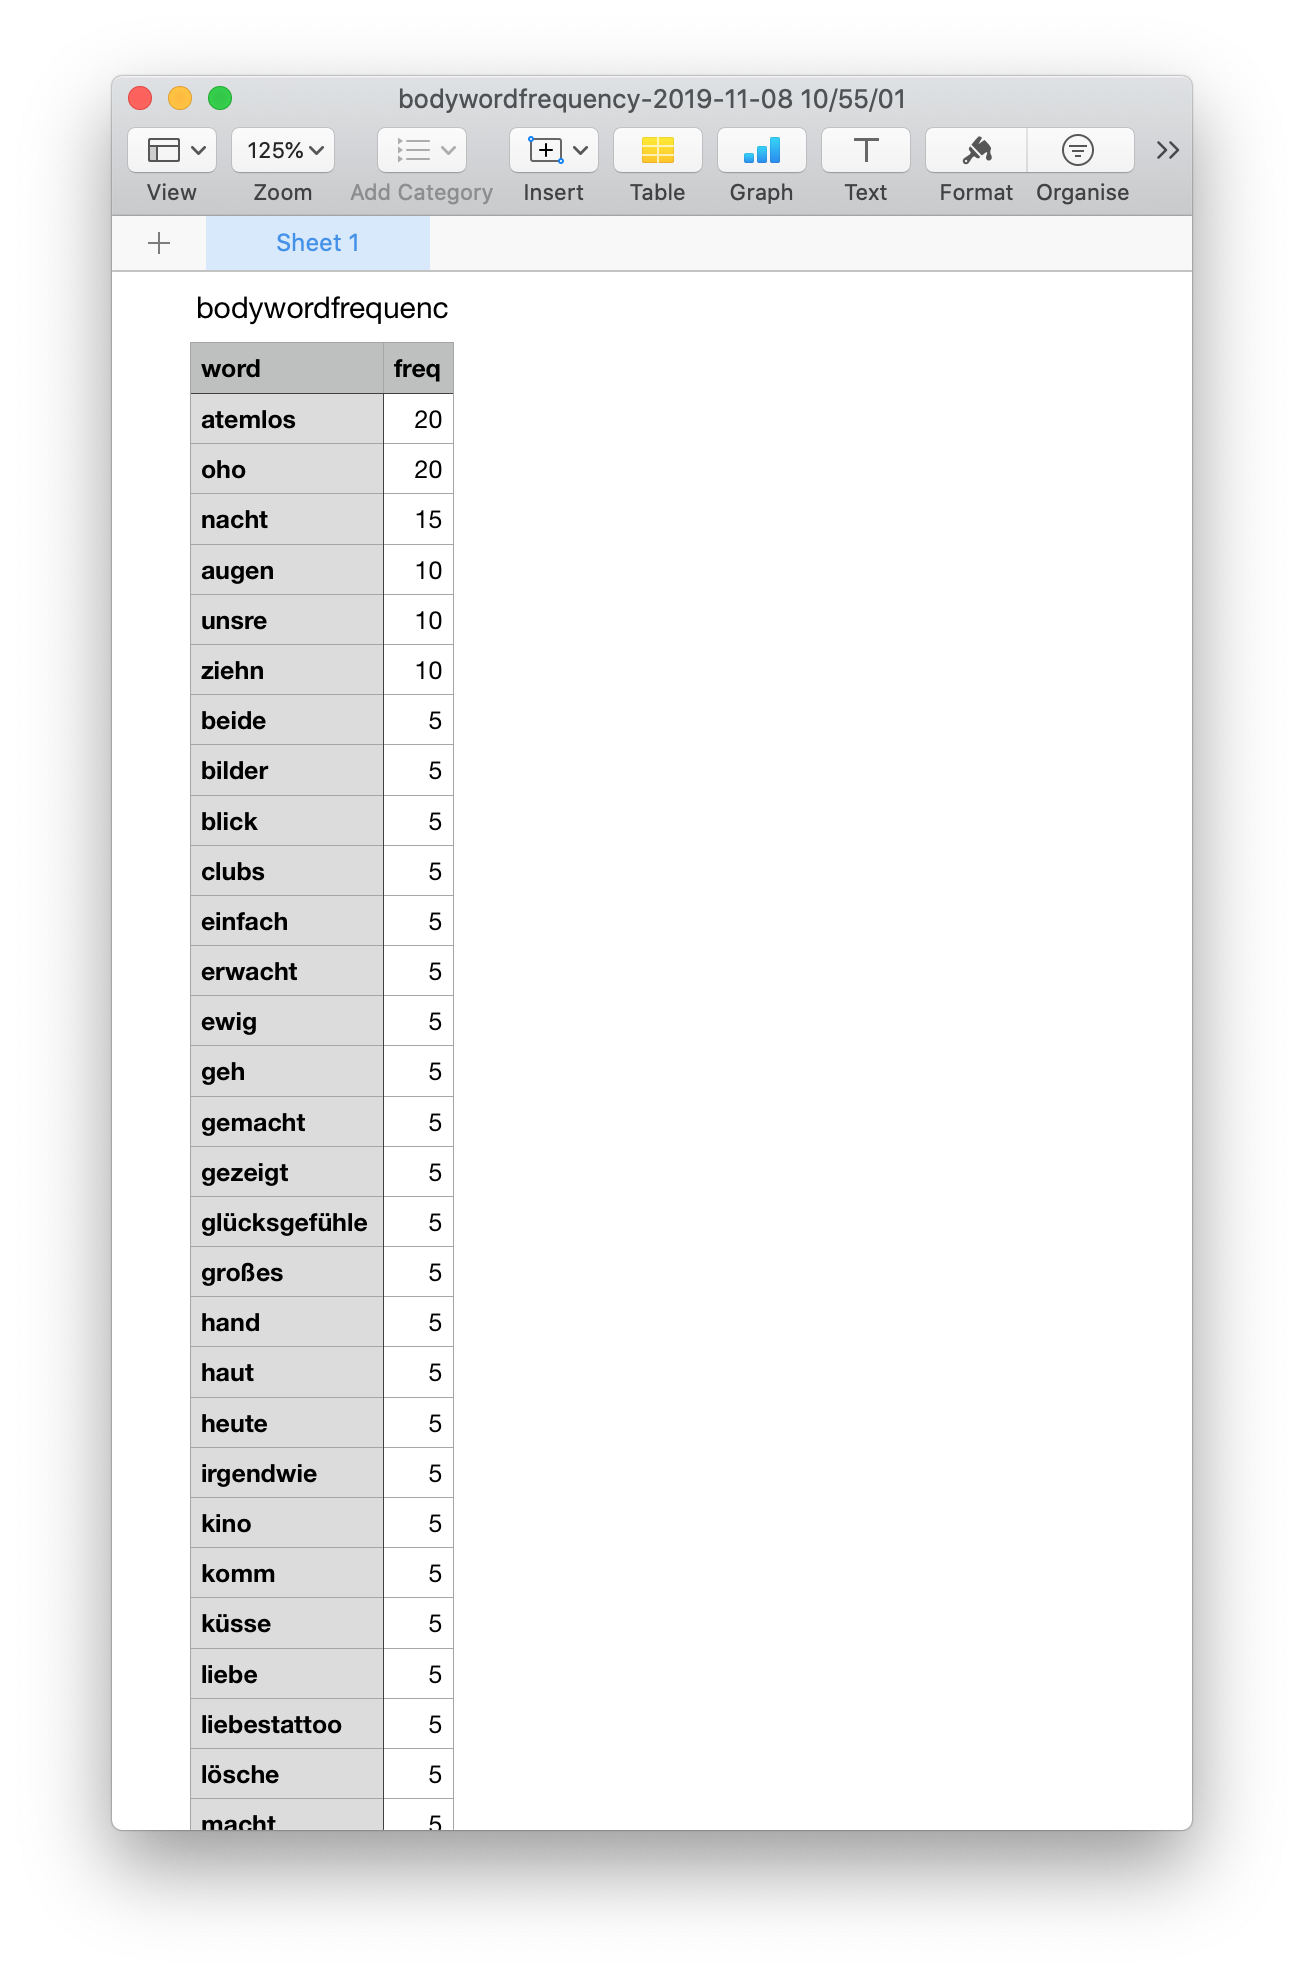
\includegraphics[width=\textwidth]{uat07.png}

Results from the title text frequency analysis are below.

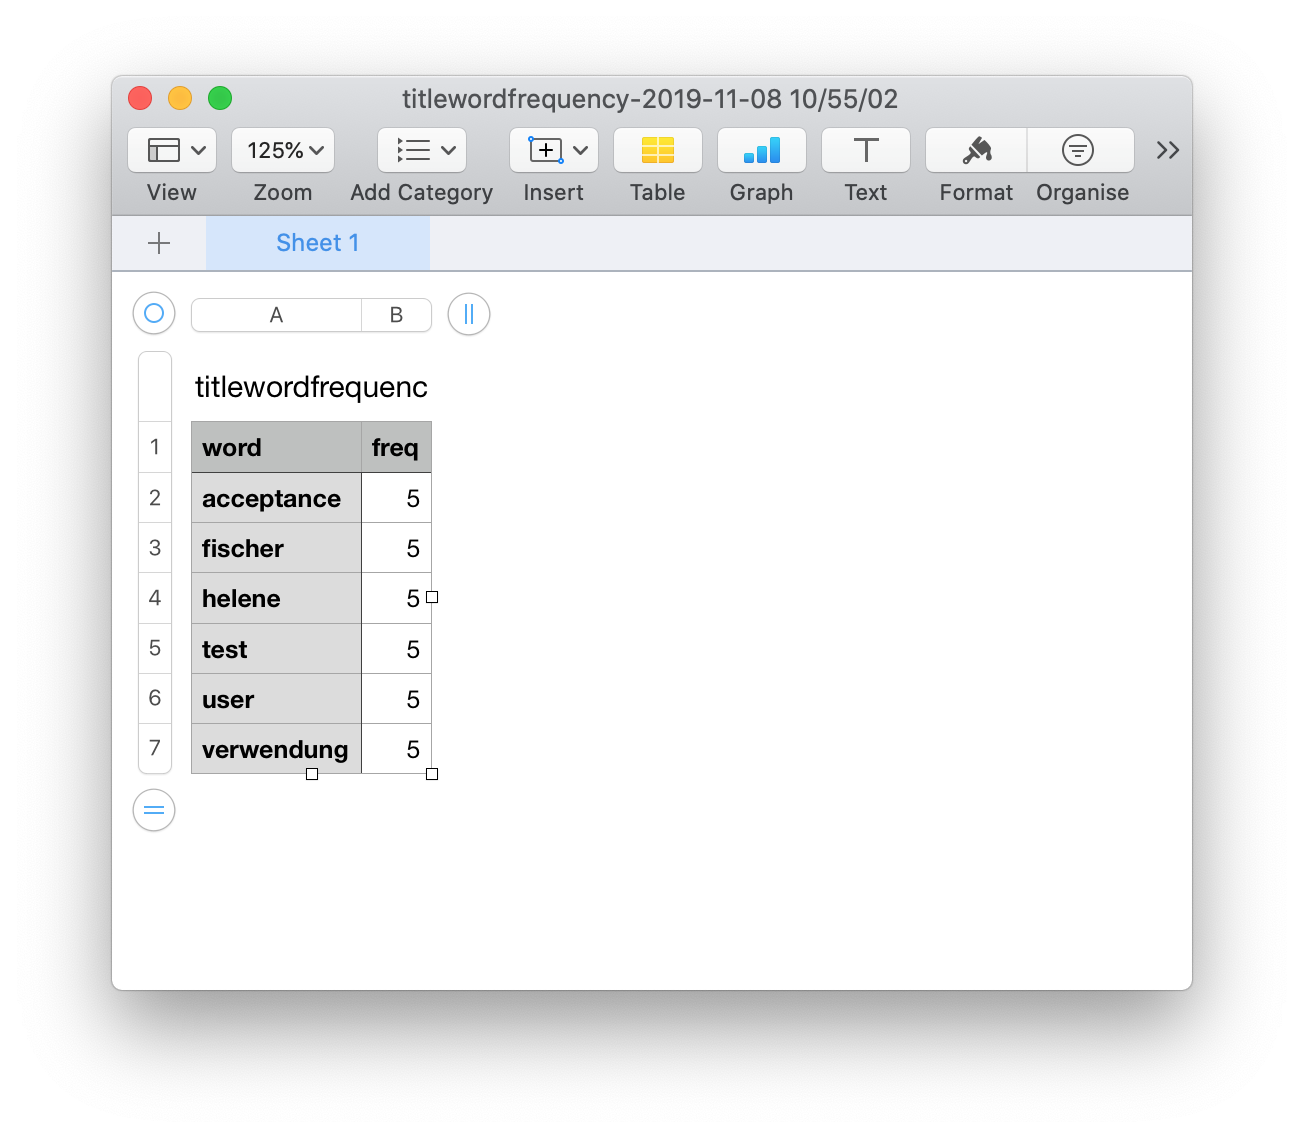
\includegraphics[width=\textwidth]{uat08.png}

Results from the title and subtitle text frequency analysis are below.

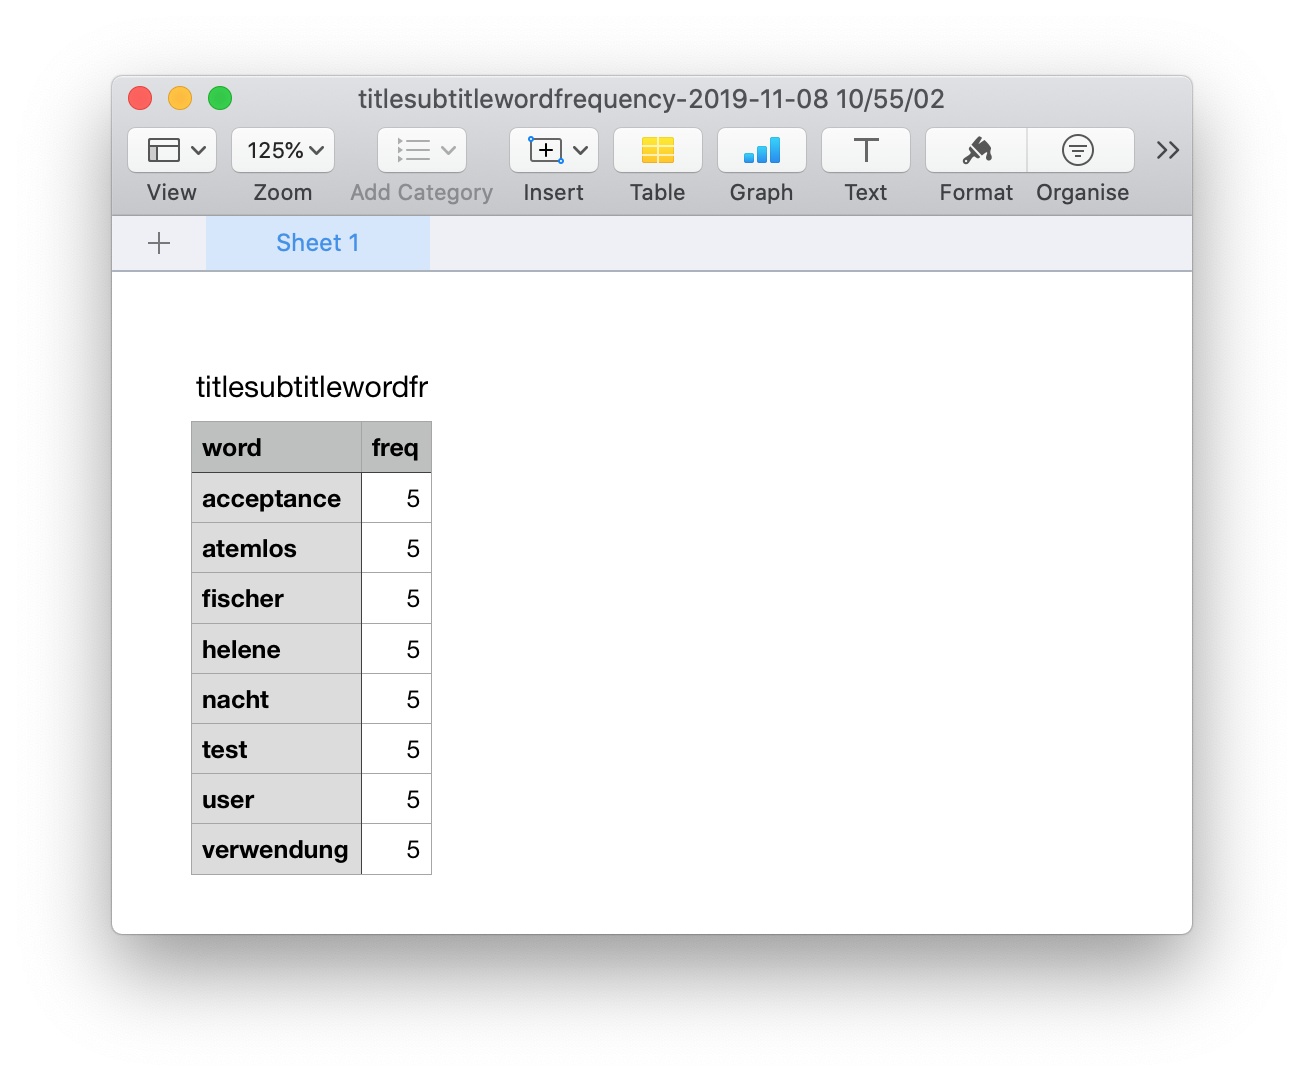
\includegraphics[width=\textwidth]{uat09.png}

The UAT Criteria have been met. The UAT has been passed.

\end{document}
